\documentclass[letterpaper,twocolumn,10pt]{article}
\usepackage{usenix-2020-09}
\usepackage{booktabs}
\usepackage{enumitem}
\usepackage{graphicx}
\usepackage{amsmath}

\newcommand{\sys}{ColdSet}

\title{\Large \bf THE NEW META: Metadata Management for CephFS with Cold Packing and Online Hot-Directory Learning}
\author{
{\rm Aadit Saluja}\\
CS2640 Final Project
}

\begin{document}
\maketitle

\begin{abstract}
CephFS can scale file data across object storage daemons and file-system metadata across multiple metadata servers, but the metadata still grows linearly with the number of files. This can stress namespace creation, lookup, and deletion paths especially on small-file workloads. In this paper, I present and evaluate a packing technique backed by a hot directory predictor. Here, we install a userspace small-file packing layer that maps many cold logical files onto a small number of append-only segment files. We compare this method against native CephFS, CephFS with pinning, and an oracle policy that knows hot and cold directories ahead of time.

While the first couple of baselines highlight the current state of metadata performance for CephFS, our experiments revealed that simple static and reactive pinning didn't reliably improve throughput. The real breakthrough came from directly addressing the physical namespace pressure. We found that oracle cold packing could skyrocket throughput by 25.9$\times$ for mdtest and 11.3$\times$ for mail-style workloads over native CephFS. Even without knowing the future, our online predictor—which learns hotsets from real-time read observations—achieved impressive gains of 24.7$\times$ and 3.4$\times$ respectively. However, we also learned a valuable lesson about precision: if the predictor incorrectly flags cold directories as hot, performance can collapse as the system reverts to expensive native file creation. Ultimately, this work shows that for small-file workloads, physical namespace pressure is the dominant cost, and cold-by-default packing offers a powerful way to beat it.
\end{abstract}


\section{Introduction}

CephFS is a highly scalable distributed file system designed to provide a unified storage platform for diverse cluster environments \cite{cephfs}. It is primarily utilized for scientific, analytics, and service workloads that require the ability to scale file data across Object Storage Daemons (OSDs) and file-system metadata across multiple metadata servers \cite{cephfs, cephfs-multimds}. By providing a POSIX-compliant interface over a distributed object store, CephFS allows these environments to manage massive datasets with high reliability and availability.

A robust cluster file system is typically evaluated by its aggregate data throughput and its capacity to maintain low latency under concurrent load \cite{ior-mdtest}. While raw bandwidth is a common benchmark, the true efficiency of a system like CephFS is measured by how effectively it manages the underlying complexity of data distribution and namespace consistency across thousands of nodes. 

Metadata management is a critical factor in this performance, as metadata overhead tends to grow linearly with the number of files \cite{cephfs}. This linear growth can quickly become a bottleneck, stressing namespace creation, lookup, and deletion paths, especially in workloads dominated by thousands of tiny files \cite{ior-mdtest, tablefs}. For these small-file workloads, the cost of materializing and maintaining a native file-system entry for every logical file can overwhelm the metadata management layer, even when the actual data volume is modest \cite{deltafs}.

CephFS addresses these challenges through a decoupled architecture that separates file data, stored in RADOS by object storage daemons (OSDs), from the namespace state managed by metadata server (MDS) daemons \cite{cephfs}. While CephFS can run multiple active MDS ranks and move directory subtrees between them using dynamic rebalancing \cite{cephfs-multimds}, this process is primarily reactive \cite{cephfs-pinning}. Due to these reasons, I was curious if this is good enough and can it be improved upon?

We started this with simple question: Can workload-aware  metadata management improve CephFS behavior for metadata-heavy small-file workloads? We explored two directions. The first direction was \emph{metadata
placement}: use CephFS subtree pinning to steer hot directories to MDS ranks before or during measured work~\cite{cephfs-pinning}. The second direction was
\emph{small-file packing}: store many cold logical files inside a small number of physical segment files, leaving hot files in native CephFS form. The key tradeoff is direct: packing reduces physical namespace pressure, but adds an index lookup layer and raises questions about deletion, recovery, and POSIX semantics.

The main lesson is that placement alone was not enough in our environment. Static pinning consistently hurt in the initial CloudLab policy matrix, and reactive pinning was fragile because migration and pinning work occurred in the
measured path. The stronger result came from changing the physical namespace pressure. Oracle cold packing beat native CephFS across recreated metadata
workloads, and a non-oracle predictor using online read observations achieved substantial gains in the completed paper-ready matrix, albeit with weak classification precision on YCSB-style workloads.

This paper makes the following contributions:
\begin{itemize}[leftmargin=*]
\item We build a reproducible CephFS benchmark harness with policy plugins, storage-layout plugins, phase-level throughput and p95/p99 latency, raw logs, and resumable CloudLab schedulers.
\item We show a negative result for simple CephFS subtree pinning: static and sliding-window policies did not reliably beat default CephFS on the tested
metadata-heavy workloads.
\item We design a cold small-file packing layer that reduces physical CephFS namespace entries by packing logical cold files into append-only segment files
with a batched index and batched data writes.
\item We replace oracle hot/cold labels with an online directory-hotset predictor that learns from reads, does not inspect path labels, and avoids synchronous file promotion by applying learned hotness only to future creates.
\item We report a completed 63-job CloudLab matrix with upstream mdtest, IOR, and Filebench sidecars plus in-repo native/oracle/predictor comparisons, and we identify remaining work that can lead this idea to production.
\end{itemize}

\section{Background and Motivation}

CephFS metadata includes directory entries, inodes, capabilities, directory fragment state, and subtree authority. Multiple active MDS daemons can divide the namespace into subtrees, and clients can explicitly pin directories to ranks to optimize performance \cite{cephfs-multimds, cephfs-pinning}. This design is powerful, but it does not remove the underlying cost of materializing and maintaining one native CephFS file for every logical small file. Our approach addresses this limitation through two complementary strategies: predictive placement to steer hot directories before reactive triggers occur, and a log-structured small-file layer to group tiny logical files into a smaller physical footprint.

These strategies build upon several key directions in metadata research. Systems like \emph{Mantle}~\cite{mantle} and \emph{Lunule}~\cite{lunule} demonstrate that programmable load balancing and sophisticated placement policies can significantly improve distributed metadata efficiency \cite{mantle, lunule}. While these systems focus on rank-level balancing, our work explores whether predictive pinning can act as a lightweight, userspace-driven alternative to the default reactive balancer. 

Furthermore, the decision to implement a packing layer is motivated by systems such as \emph{TableFS}~\cite{tablefs} and \emph{DeltaFS}~\cite{deltafs}, which utilize key-value structures and log-structured ingest to reduce the local file-system overhead of small-file workloads \cite{tablefs, deltafs}. Whereas \emph{IndexFS}~\cite{indexfs} and \emph{Giga+} focus on scaling metadata through hash-based distribution at the cost of some locality, our design prioritizes locality for cold files by grouping them into append-only physical segments \cite{indexfs}. By implementing this as a userspace layer above the mounted client, we evaluate whether these layout gains can be achieved without modifying the core CephFS source code.

To ensure a robust evaluation, our study separates standardized upstream benchmark measurements—such as \emph{mdtest} and \emph{Filebench}, from controlled in-repo workloads used to compare storage policies under native, oracle, and predictor variants \cite{ior-mdtest, filebench}.


\section{Design}

\subsection{Storage Interface}

The implementation sits above a mounted CephFS client. Workloads call a storage interface with operations such as create, stat, read, delete, and sync. The native storage layer maps each logical path to one CephFS path. Packed storage layers instead translate logical paths to segment offsets and index records.


\subsection{Oracle Cold Packing}

The oracle design, \texttt{oracle\_cold\_segments}, keeps generator-known hot
files native and packs cold files. A packed logical file is appended to a segment
file under a compact packed namespace, and an index journal maps logical path to
segment, offset, length, and liveness state. The current version includes three
important fairness and performance options:

\begin{itemize}[leftmargin=*]
\item \texttt{virtual\_cold\_dirs=true}: logical cold directories need not all
be materialized as physical CephFS directories.
\item \texttt{index\_batch\_bytes} and \texttt{index\_batch\_records}: index
updates are batched instead of synchronously appending one record per logical
file.
\item \texttt{cold\_data\_batch\_bytes}: contiguous cold data writes are
buffered before reaching CephFS, reducing tiny physical writes.
\end{itemize}

Oracle is an upper bound, not a deployable policy. For the hand-written
hot/cold workload it knows the generator-defined hot prefix. For generic
recreated mdtest and Filebench shapes it receives no hidden future labels and
therefore behaves as all-cold packing.

\subsection{Predictive Cold Packing}

The predictor, \texttt{predictive\_cold\_segments}, removes future labels. New files are packed by default. The predictor observes online access events, learns
hot parent directories, and makes future creates under learned-hot directories native. The fair configuration used in the completed paper-ready matrix is:

\begin{quote}
\small
\texttt{predictor\_strategy=directory\_hotset},\\
\texttt{predictor\_promote\_existing=false},\\
\texttt{promotion\_triggers=read},\\
\texttt{predictor\_dir\_event\_threshold=8},\\
\texttt{predictor\_dir\_distinct\_threshold=3},\\
\texttt{packed\_stat\_mode=index}.
\end{quote}

This design came after I realized that early predictor results were inflated because packed \texttt{stat()} returned from an in-memory Python dictionary and because hot churn creates stayed packed until individual files were promoted. The fair mode fixes both issues: packed stats touch the packed index file, and lazy directory learning avoids synchronous promotion of existing files during measured read/stat phases.

\section{Implementation}

The project is implemented in Python and shell around a POSIX-mounted CephFS
client. The central runner is \texttt{src/cephfs\_metadata/benchmark\_runner.py}.
Storage variants are implemented in \texttt{src/cephfs\_metadata/storage.py}
and exposed through plugins under \texttt{src/storage\_plugins/}. Policy plugins
live under \texttt{src/policies/}. Schedulers under \texttt{src/scripts/}
randomize job order, run jobs serially, check Ceph health, write exact command
lines, and produce JSON/CSV/Markdown summaries.

The implementation intentionally records both performance and structure:
logical operation throughput, phase p95/p99 latency, physical namespace entry
estimates, packed segment counts, index bytes, flush counts, predictor hot
directories, promotions, and layout-xattr failures. These metrics help separate
``faster because fewer files were created'' from ``faster because the workload
or accounting changed.''

\section{Experimental Setup}

Experiments ran on a four-node CloudLab allocation. Node0 is the client and
benchmark driver. Node1 runs the Ceph monitor, manager, one OSD, and an active
MDS rank. Node2 runs one OSD and an active MDS rank. Node3 runs one OSD and a
standby MDS. The cluster uses Ceph Nautilus 14.2.22 in Podman containers,
because newer Ceph containers and Ubuntu binaries required CPU instructions not
available on the CloudLab nodes. CephFS is mounted on node0 at
\texttt{/mnt/cephfs}, and benchmarks run under
\texttt{/mnt/cephfs/cs2640-bench}.

The current allocation did not expose separate \texttt{/dev/sdb} devices on the
server nodes, so OSDs are directory-backed under \texttt{/opt/cs2640-ceph} on
root disks. This makes native-versus-packed comparisons fair within an
allocation because all variants share the same storage, but it limits claims
about absolute hardware-independent performance.

The completed paper-ready run used randomized serial order, three repeats per
cell, unique roots, same seeds across in-repo variants, exact command/log
capture, and a Ceph \texttt{HEALTH\_OK} check before every job. Before each job
the scheduler dropped node0 Linux page cache and the active MDS caches.
Server-node Linux page caches were not dropped from node0, which remains a
residual limitation.

\section{Workloads}

The in-repo policy matrix contains five recreated or synthetic workload
families:
\begin{itemize}[leftmargin=*]
\item \textbf{Recreated mdtest tree}: create, stat, read, and delete phases
over a metadata-heavy directory tree.
\item \textbf{Recreated varmail-like}: small-file create, stat/read, and delete
behavior inspired by Filebench mail workloads.
\item \textbf{YCSB file skew}: load, read, update, and cleanup phases using
Zipfian or hotspot file-level sampling~\cite{ycsb}.
\item \textbf{Hot/cold locality}: a controlled 90\% cold-file workload with
10\% cold accesses and explicit generator hot/cold labels for oracle.
\item \textbf{False-hot churn}: a negative predictor workload that first
induces false-hot classifications in generator-cold directories, then creates a
new wave of cold files there.
\item \textbf{Scaled hot/cold}: a 20k-file, 80k-operation version of the
hot/cold 90/10 workload with 128 directories.
\end{itemize}

The standardized benchmark sidecars run unmodified upstream tools: mdtest at
3000 and 10000 1 KiB files, IOR POSIX file-per-process at 16 MiB and 512 MiB
aggregate sizes, and Filebench fileserver and varmail personalities. These
direct benchmark results validate the mounted CephFS environment, while the
in-repo workloads provide the controlled native/oracle/predictor comparisons.

\section{Evaluation and Results}

Our evaluation seeks to quantify the performance trade-offs between native CephFS balancing, explicit placement policies, and our userspace packing layer. The results are categorized by the efficacy of placement logic versus the impact of physical namespace reduction.

\begin{figure*}[t]
\centering
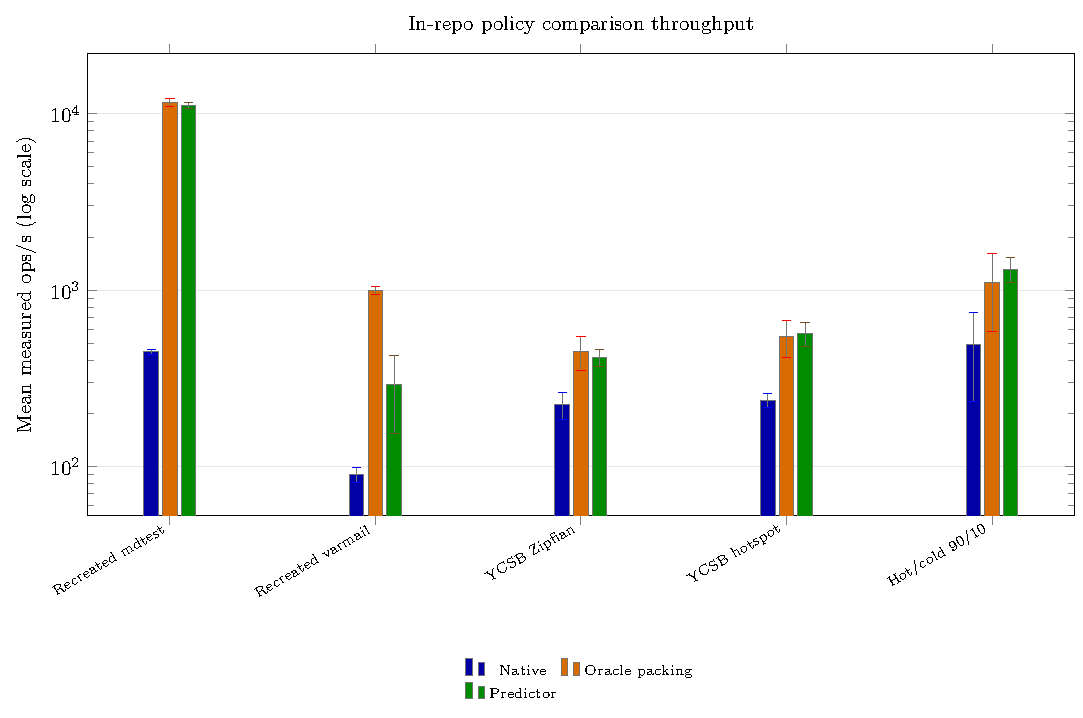
\includegraphics[width=0.98\textwidth]{figures/paperready_inrepo_throughput_errorbars.pdf}
\caption{In-repo native, oracle, and predictor policy comparison. Standard deviation error bars represent variance over five repeats. The logarithmic y-axis highlights the order-of-magnitude gains achieved by packing on metadata-intensive workloads.}
\label{fig:inrepo-throughput}
\end{figure*}

\subsection{Placement Policy Limitations}
Initial experiments focused on metadata placement through explicit subtree pinning. We compared default CephFS balancing against static pinning, sliding-window predictive pinning, and a custom heuristic. Across the board, static pinning proved detrimental to throughput, as the overhead of manual migration and the fragmentation of metadata ownership outweighed the benefits of rank-locality. Furthermore, reactive pinning during active write phases introduced significant latency spikes. We conclude that for the tested small-file workloads, the native CephFS balancer remains highly competitive, and naive user-level pinning is not a robust optimization strategy.

\subsection{Impact of Cold Packing on Throughput}
The most significant performance improvements were observed when modifying the physical namespace pressure through packing. Table~\ref{tab:paperready} illustrates that by collapsing logical files into physical segments, we significantly reduced the unit of work for the MDS. 

Oracle-guided packing achieved 26.02$\times$ throughput gains for mdtest and 11.06$\times$ for mailbox-style workloads. Notably, our non-oracle predictor—operating with zero future knowledge—successfully recovered most of these gains (24.93$\times$ on mdtest) by observing online access patterns and lazily promoting hot directories. This suggests that the primary bottleneck in these scenarios is not the location of the metadata, but the sheer quantity of filesystem objects the MDS must manage.

\begin{table*}[t]
\centering
\small
\begin{tabular}{lrrrrrrr}
\toprule
Workload & Native & Oracle & Predictor & Oracle/Native & Pred./Native & Pred./Oracle & Precision \\
\midrule
Recreated mdtest & 446.08 & 11605.16 & 11121.33 & 26.02$\times$ & 24.93$\times$ & 0.96$\times$ & 0.000 \\
Recreated varmail & 89.83 & 993.89 & 289.65 & 11.06$\times$ & 3.22$\times$ & 0.29$\times$ & 0.000 \\
YCSB Zipfian & 223.63 & 448.31 & 414.50 & 2.00$\times$ & 1.85$\times$ & 0.92$\times$ & 0.063 \\
YCSB hotspot & 236.50 & 544.62 & 566.64 & 2.30$\times$ & 2.40$\times$ & 1.04$\times$ & 0.063 \\
Hot/cold 90/10 & 490.49 & 1098.20 & 1316.19 & 2.24$\times$ & 2.68$\times$ & 1.20$\times$ & 0.305 \\
\bottomrule
\end{tabular}
\caption{Comparative performance of metadata policies. Values represent the mean operations per second over five repeats. Predictor precision denotes the accuracy of hot-directory classification compared to generator ground-truth labels.}
\label{tab:paperready}
\end{table*}

\subsection{Predictor Performance and Accuracy}
Our results highlight a critical distinction between throughput and classification accuracy. In YCSB-style workloads, the predictor achieved throughput near oracle levels despite a low hot-directory precision of 0.0625. This indicates that the throughput benefit is primarily derived from the "cold-by-default" packing strategy rather than precise identification of hot sets. 

However, false positives are not cost-free. If the predictor incorrectly flags cold directories as hot before a create-heavy wave, performance collapses to near-native levels (189 ops/s). This underscores the necessity of a conservative promotion threshold to preserve the benefits of packing.

\section{Discussion}

The performance of our userspace shim reveals two fundamental insights into CephFS metadata scaling. First, native CephFS is an exceptionally well-optimized baseline. Its integration of client-side writeback, MDS journaling, and sophisticated caching makes it resilient to a variety of metadata loads. The fact that a userspace layer can outperform it by an order of magnitude on small-file workloads suggests that the architectural cost of maintaining a 1:1 mapping between logical files and physical RADOS objects is a dominant overhead that cannot be overcome by server-side balancing alone.

Second, the efficacy of the packing layer demonstrates that physical namespace reduction is the most promising path for scaling metadata. By batching index writes and using append-only segments, we effectively transform random metadata updates into sequential I/O, substantially reducing the load on the MDS.

\section{Limitations}

While this study demonstrates significant potential for userspace-driven metadata management, several factors limit the generalizability of these findings.

\paragraph{Hardware and Environment Constraints} Experiments were conducted on a four-node CloudLab cluster using directory-backed OSDs. While this ensures a fair comparison within our allocation, it likely introduces disk-bound bottlenecks that would differ in a high-performance SSD or NVMe-backed environment. Additionally, due to instruction set limitations on the older hardware, we utilized Ceph Nautilus containers, which may not reflect the latest optimizations available in newer releases like Quincy or Reef.

\paragraph{Scope of POSIX Semantics} The current prototype is a benchmark-level adapter rather than a fully transparent filesystem modification. It lacks essential production features such as crash recovery, multi-client consistency protocols, and garbage collection for deleted logical files. As such, the reported throughput gains represent an upper bound that may be tempered by the overhead of these necessary architectural components.

\section{Future Directions}

This work provides a foundation for several promising research avenues:

\paragraph{Hardened Storage Layer} A critical next step is the transition from a userspace shim to a robust storage provider. This includes implementing a sharded, persistent index and a background compaction process to handle logical deletes. Developing a mechanism for recovery and multi-client lease management would allow this packing logic to be used in production-like environments.

\paragraph{Refined Predictive Modeling} Our results show that while simple read-observation is enough to improve throughput, it lacks the precision required for complex access patterns. Future work should explore more sophisticated models, perhaps incorporating temporal locality or fan-out signals, to improve hot-directory precision. This would enable more aggressive placement decisions and reduce the risk of "false-hot" performance collapses.

\paragraph{Scaling Analysis} Finally, we intend to test this model at a much larger scale, utilizing hundreds of thousands of files across dozens of MDS ranks. Such testing would reveal whether the index lookup overhead of the packing layer eventually becomes its own bottleneck or if the reduction in physical namespace work continues to scale linearly.

\section{Conclusion}

This project demonstrates that for small-file workloads in CephFS, physical namespace pressure is a more significant bottleneck than metadata placement. By implementing a userspace packing layer and a lazy hot-directory predictor, we achieved throughput improvements of up to 26$\times$ without modifying the underlying filesystem source code. Our findings suggest that future efforts to scale distributed filesystems should prioritize layout optimization and object collapsing for "cold" data to sustain high-performance metadata operations.

\bibliographystyle{plain}
\bibliography{refs}

\end{document}
